\setcounter{secnumdepth}{4}
\titleformat{\paragraph}
{\normalfont\normalsize\bfseries}{\theparagraph}{1em}{}
\titlespacing*{\paragraph}
{0pt}{3.25ex plus 1ex minus .2ex}{1.5ex plus .2ex}

\section{2D 2G Quarter Core}
\subsection{Equations}
This problem is a more traditional $k$-eigenvalue criticality problem using neutron diffusion.  We simulate a benchmark reactor core by imposing reflecting conditions on the left and bottom boundaries of a quarter-core geometry.  The governing PDE for this equation is still
\begin{equation}
-\drv{}{x}D_g\drv{\phi_g}{x}+(\Sigma_{g,a}+\Sigma_{g,s})\phi_g = \sum_{g'}\sigma_{s}^{g'\to g}\phi_{g'} + \frac{\chi_{g}}{k}\sum_{g'}\nu_{g'}\sigma_{f,g'}\phi_{g'},\hspace{15pt} g\in[1,2],
\end{equation}
\begin{equation}
\Sigma_{g,a}=\Sigma_{g,c}+\Sigma_{g,f},
\end{equation}
where $g$ denotes the energy group, $D$ is the group diffusion cross section; $\phi$ is the group flux, $x$ is the location within the problem; $\Sigma_a,\Sigma_s,\Sigma_f$ are the macroscopic absorption, scattering, and fission cross sections respectively; $k$ is the criticality factor eigenvalue and quantity of interest; and $\chi$ is the fraction of neutrons born into an energy group.  In this case, we consider only downscattering, and fission neutrons are only born into the high energy group ($\Sigma_s^{2\to1}=\chi_2=0$).  Our coupled equations are
\begin{equation}
-\drv{}{x}D_1\drv{\phi_1}{x}+(\Sigma_{1,a}+\Sigma_s^{1\to2})\phi_1 = \frac{1}{k}\sum_{g'=1}^2\nu_{g'}\sigma_{f,g'}\phi_{g'},
\end{equation}
\begin{equation}
-\drv{}{x}D_2\drv{\phi_2}{x}+\Sigma_{2,a}\phi_2 = \sigma_{s}^{1'\to 2}\phi_1,
\end{equation}
\begin{equation}
\Sigma_{g,a}=\Sigma_{g,c}+\Sigma_{g,f}.
\end{equation}

\subsection{Materials and Geometry}
The two-dimensional core is shown in Fig. \ref{coremap} and the material properties are listed in Table \ref{tab:coremats}.
\begin{figure}[H]
\centering
   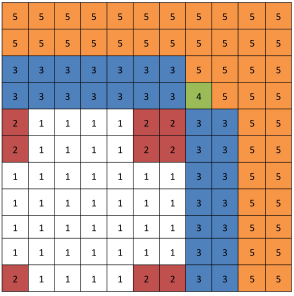
\includegraphics[width=0.4\textwidth]{../graphics/core}
   \caption{Core Map}
   \label{coremap}
\end{figure}
\begin{table}[H]
\centering
\begin{tabular}{c c | c c c c}
Region & Group & $D_g$ & $\Sigma_{c,g}$ & $\nu\Sigma_{f,g}$ & $\Sigma_s^{1,2}$ \\ \hline
1 & 1 & 1.255    & 4.602e-3 & 4.602e-3 & 2.533e-2 \\
  & 2 & 2.11e-1  & 5.540e-2 & 1.091e-1 & \\ \hline
2 & 1 & 1.268    & 4.609e-3 & 4.609e-3 & 2.767e-2 \\
  & 2 & 1.902e-1 & 8.675e-2 & 8.675e-2 & \\ \hline
3 & 1 & 1.259    & 6.083e-3 & 4.663e-3 & 2.617e-2 \\
  & 2 & 2.091e-1 & 4.142e-2 & 1.021e-1 & \\ \hline
4 & 1 & 1.259    & 4.663e-3 & 4.663e-3 & 2.617e-2 \\
  & 2 & 2.091e-1 & 3.131e-2 & 1.021e-1 & \\ \hline
5 & 1 & 1.257    & 6.034e-4  & 0 & 4.754e-2 \\
  & 2 & 1.592e-1 & 1.911e-2  & 0 & 
\end{tabular}
\caption{Basic Material Properties for Core}
\label{tab:coremats}
\end{table}

\subsection{Uncertainty Quantification}
\subsubsection{Univariate}
This problem also does not have a convenient general analytic solution.  We can express the solver as
\begin{equation}
U(p;\theta) = k(p;\Sigma_{2,c}),
\end{equation}
where
\begin{equation}
p=(D_g,\Sigma_{1,c},\Sigma_{g,s},\nu_g,\Sigma_{g,f},\chi_g),\hspace{20pt}g\in[1,2].
\end{equation}
While $\phi_g(x)$ might also be considered a parameter, it is an output value solved simultaneously with $k$.

\paragraph{Uniform Uncertainty}
For this test we consider $\theta=\Sigma_{2,c}$ uniformly distributed as $\theta\in\mathcal{N}(0.0454,0.0654s)$. Tabular data for mean and variance convergence is in Table \ref{tab:2dcrit uni}, and the pdfs obtained are in Fig. \ref{fig:2dcrit uni}.

The PCESC runs all made use of order 32 quadrature to integrate chaos moments.

\begin{table}[H]
\begin{center}
\begin{tabular}{c c|l l}
type & runs/order & mean & variance \\ \hline
MC & $1\times10^6$ & 1.00406413634 & 0.000446173081079 \\
SC & 2  & 1.00416405471 & 0.000375112851817 \\
SC & 4  & 1.00416405471 & 0.000390962150246 \\
SC & 8  & 1.00416405471 & 0.000406864600682 \\
SC & 16 & 1.00416405471 & 0.000421349517322 \\
SC & 32 & 1.00416405471 & 0.000425027572716
\end{tabular}
\end{center}
\caption{Convergence of Mean, Variance for 2D2G Case}
\label{tab:2dcrit uni}
\end{table}

\begin{figure}[H]
\centering
   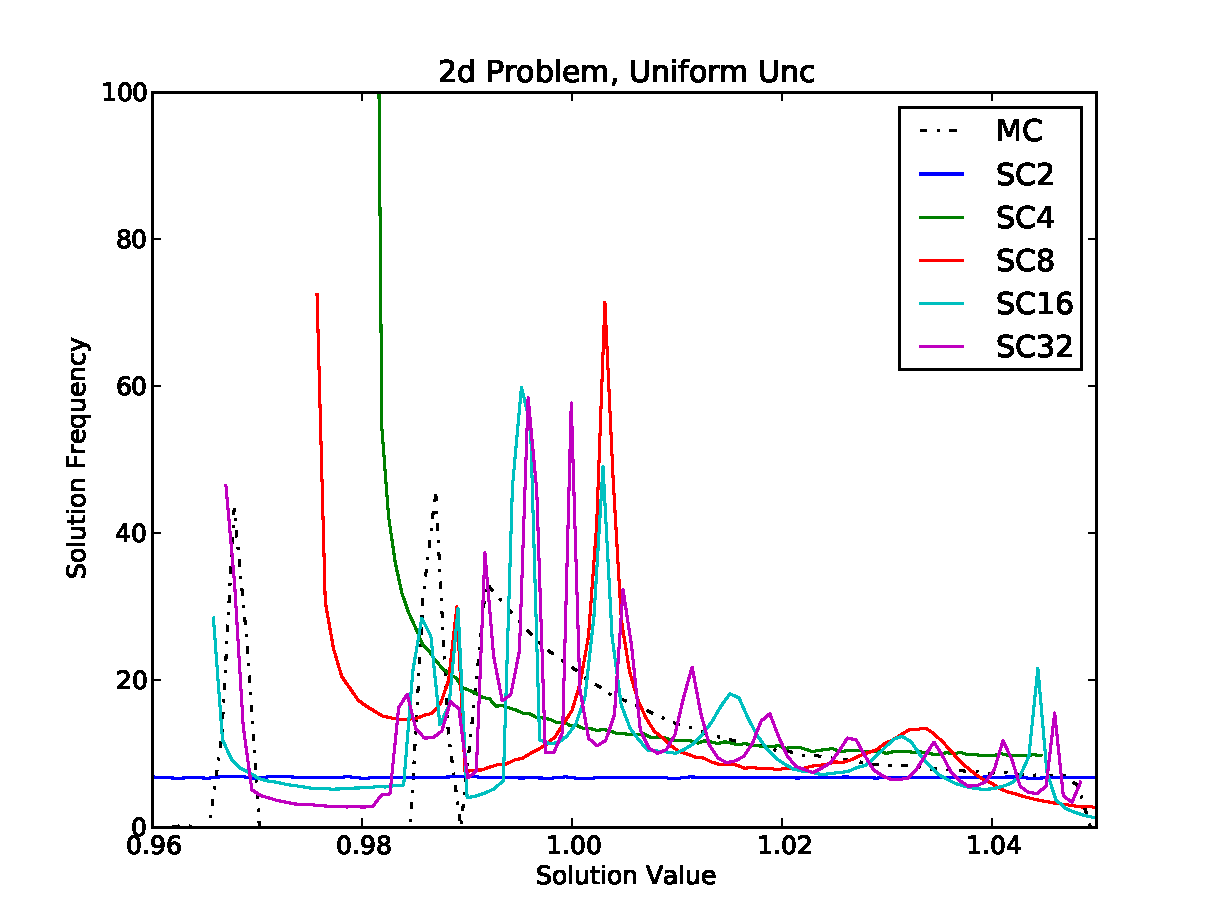
\includegraphics[width=\textwidth]{../graphics/2d_uniform_pdfs}
   \caption{Solution PDF Convergence, 2D2G Case}
   \label{fig:2dcrit uni}
\end{figure}

\paragraph{Normal Uncertainty}
For this test we consider $\theta=\Sigma_{2,c}$ normally distributed as $\theta\in\mathcal{N}(0.0554,0.01^2)$. Tabular data for mean and variance convergence is in Table \ref{tab:2dcrit}, and the pdfs obtained are in Fig. \ref{fig:2dcrit}.  Once again, it is important to note that the Monte Carlo sampling was restricted to values within 3 standard deviations of the mean; as such, the means and variances obtained directly through Monte Carlo sampling are not representative of the full uncertainty space.  This truncation of the distribution is enforced because without such a restriction, it is possible to sample physically untenable values for $\Sigma_{2,c}$, including negative values.

The PCESC runs all made use of order 32 quadrature to integrate chaos moments.

\begin{table}[H]
\begin{center}
\begin{tabular}{c c|l l}
type & runs/order & mean & variance \\ \hline
MC & $6\times10^5$ & 1.01333702129 & 0.00160652595587 \\
SC & 2  & 1.01643813464 & 0.00138703446968 \\
SC & 4  & 1.01643813464 & 0.00184314998697 \\
SC & 8  & 1.01643813464 & 0.00184690058216 \\
SC & 16 & 1.01643813464 & 0.00184724103523 \\
SC & 32 & 1.01643813464 & 0.00184726152781
\end{tabular}
\end{center}
\caption{Convergence of Mean, Variance for 2D2G Case}
\label{tab:2dcrit}
\end{table}

\begin{figure}[H]
\centering
   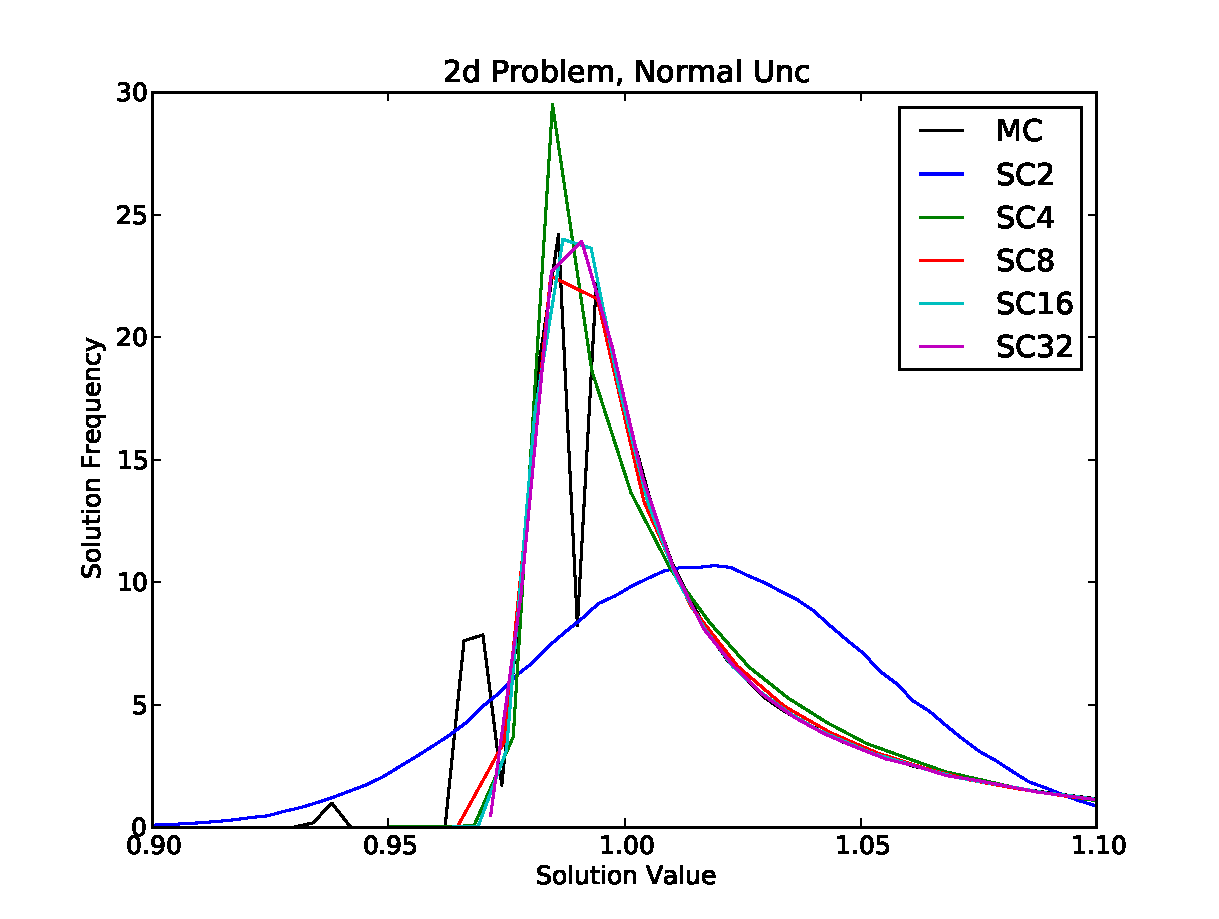
\includegraphics[width=\textwidth]{../graphics/2d_normal_pdfs}
   \caption{Solution PDF Convergence, 2D2G Case}
   \label{fig:2dcrit}
\end{figure}

\subsubsection{Multivariate}
In this case we consider five uncertain parameters simultaneously, as in Table \ref{tab:2d2g5param}.  Each was given approximately 10\% uncertainty from its mean in the benchmark problem.
\begin{table}
\begin{center}
\begin{tabular}{c c c c}
Region & Energy Group & Parameter & Uncertainty \\ \hline
1 & 2 & $\Sigma_c$ & $\mathcal{U}(0.050,0.061) $\\
1 & 2 & $\Sigma_f$ & $\mathcal{U}(0.098,0.120) $\\
4 & 2 & $\Sigma_c$ & $\mathcal{U}(0.037,0.046) $\\
4 & 2 & $\Sigma_f$ & $\mathcal{U}(0.092,0.112) $\\
5 & 2 & $D$            & $\mathcal{U}(0.143,0.175) $\\
\end{tabular}
\end{center}
\caption{Multivariate Uncertainty Space}
\label{tab:2d2g5param}
\end{table}

To explore the input space, we consider a variety of low-order expansions and one of higher order.  The results are in Table \ref{tab:2dcrit5v}.

\begin{table}[H]
\begin{center}
\begin{tabular}{c c|l l}
type & $\mathcal{O}(\Sigma_{2,c}^1,\Sigma_{2,f}^1,\Sigma_{2,c}^4,\Sigma_{2,f}^4,D^5_2)$ & mean & variance \\ \hline
MC & $1\times10^6$ & 0.995950138052 & 1.34575404516 \\
SC & (2,2,2,2,2)  & 1.00261445437 & 0.000173828352441 \\
SC & (4,2,2,2,2)  & 1.00125722573 & 0.000245435396045 \\
SC & (2,4,2,2,2)  & 1.00125489157 & 0.000244969265818 \\
SC & (2,2,4,2,2)  & 1.00261445458 & 0.000173828361529 \\
SC & (2,2,2,4,2)  & 1.00261445431 & 0.000173828341974 \\
SC & (2,2,2,2,4)  & 1.00261445434 & 0.000173828350938 \\
SC & (4,4,2,2,2)  & 1.00261444028 & 0.00017376644541\\
SC & (6,6,2,2,2)  & 1.00192854415 & 0.000216430946449 \\
SC & (8,8,8,8,8) & 0.988408029125 & 1.17178207098
\end{tabular}
\end{center}
\caption{Convergence of Mean, Variance for 2D2G Case}
\label{tab:2dcrit5v}
\end{table}

\paragraph{Convergence Study}
There are several factors to consider in the selection of expansion orders for each input parameter.  To inform us on appropriate expansion orders, we first consider each input parameter separately.  Because they are independent, holding the other parameters at their means while exploring convergence in expansion order of a single parameter gives an appropriate estimate for each expansion order in a multivariate run.  To increase run speed, we reduce the mesh refinement to its coarsest level (one grid cell per region).  We use 256-order Gauss Legendre quadrature to construct 256 expansion moments for each input parameter separately.  The results are shown in Fig. \ref{fig:2g2d5v coarse cof}.  The y-axis is the log of the magnitude of the expansion coefficient, and the x-axis is the expansion moments sorted by order.  The coefficient magnitude falls of quickly over the first several terms and plateaus for each case; however, the high value plateau for the Region 1 material cross sections suggests a lack of convergence.
\begin{figure}[H]
\centering
   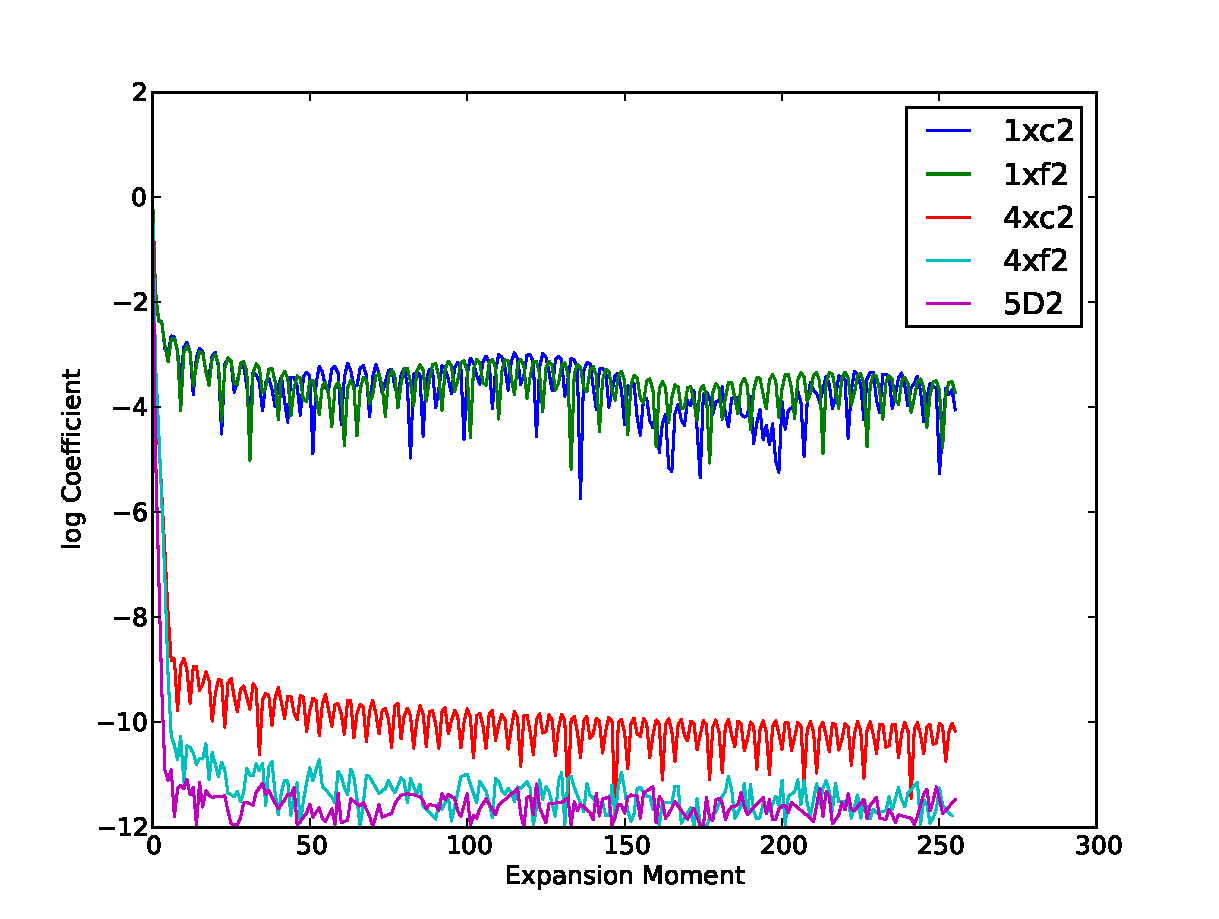
\includegraphics[width=0.7\textwidth]{../graphics/coefficient_decay}
   \caption{2G2D: Coarse Mesh Coefficient Decay}
   \label{fig:2g2d5v coarse cof}
\end{figure}
We hypothesize that this lack of convergence is because of the discretization error in the solver with such a coarse mesh.   To demonstrate the effect of increasing mesh refinement, we consider only the low-energy capture cross section for the first region (1xc2, $\xs{c}{1}$).  The results are shown in Fig. \ref{fig2g2d 1xc2 cof decay}.
\begin{figure}[H]
\centering
   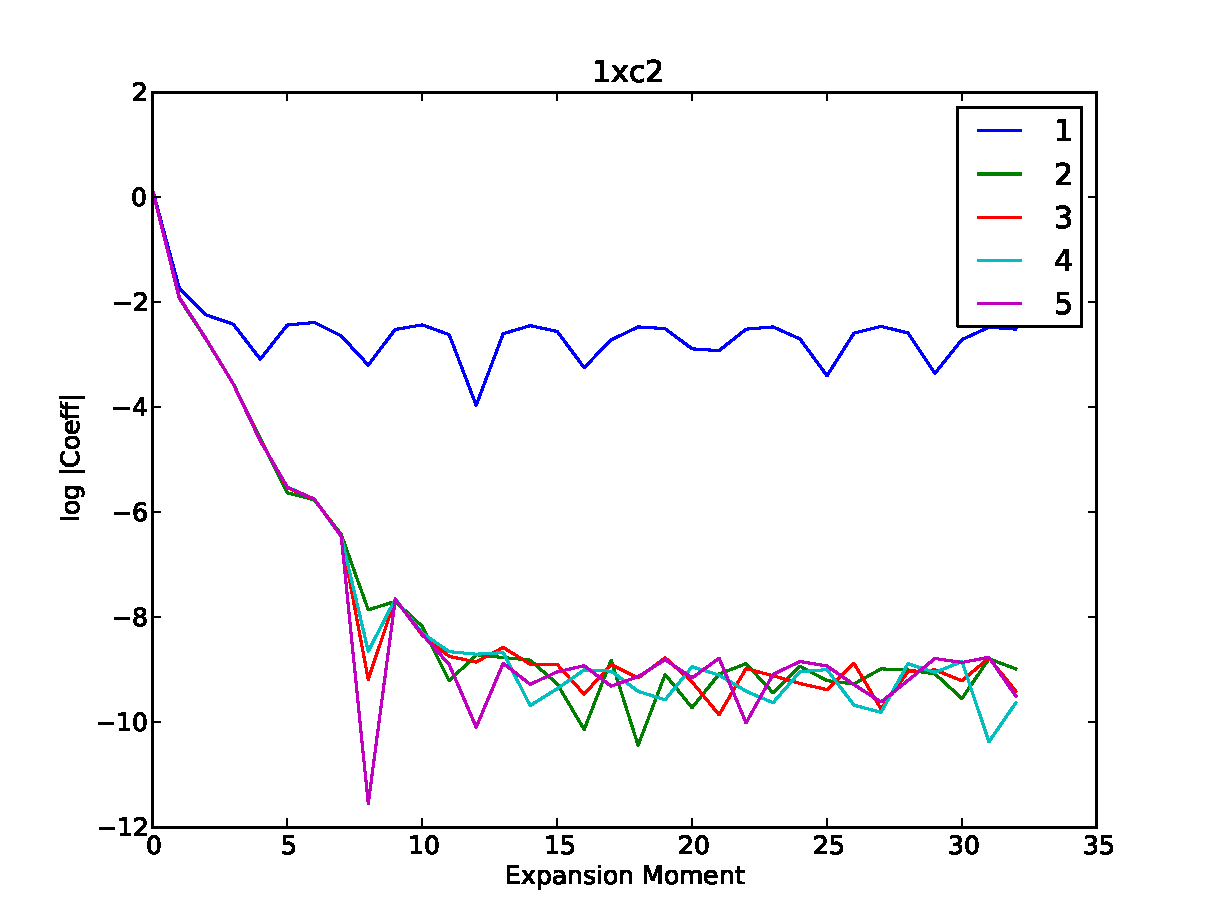
\includegraphics[width=0.7\textwidth]{../graphics/cof_decay_1xc2_meshes}
   \caption{2G2D: Coefficients over Mesh Refinement}
   \label{fig:2g2d 1xc2 cof decay}
\end{figure}
It is worth noting that any integer increase in the mesh refinement per region results in a large increase in mesh refinement overall.  The coarsest mesh, using a factor of 1 (1x1 grid cell per region) results in a mesh that is 11x11.  A mesh factor of 2 (2x2 grid cells per region) increases the refinement to 22x22.  This is equivalent to moving from $h=\Delta_x=\Delta_y=15$ cm to $h=7.5$ cm.  For this particular set of parameters, increase the mesh factor from 1 to 2 is plenty to assure good convergence for this cross section.  It can be the shown that the other Region 1 input parameter in this study behaves similarly and converges much further using a mesh factor of 2.

We perform the same convergence study as before, but using the more refined mesh and only continuing to order 32 expansions.  The results are shown in Fig. \ref{fig:2g2d5v fine cof}.  While the first region material cross sections don't converge as far as the fourth region and reflector (fifth region), they do converge much further.  Looking at this plot, we can choose a multivariate expansion order that accurately represents the system.  Table \ref{tab:informed 5v} shows the results of keeping different expansion orders chosen by imposing a coefficient convergence tolerance.  In each case, the quadrature order used is double the expansion order.
\begin{figure}[H]
\centering
   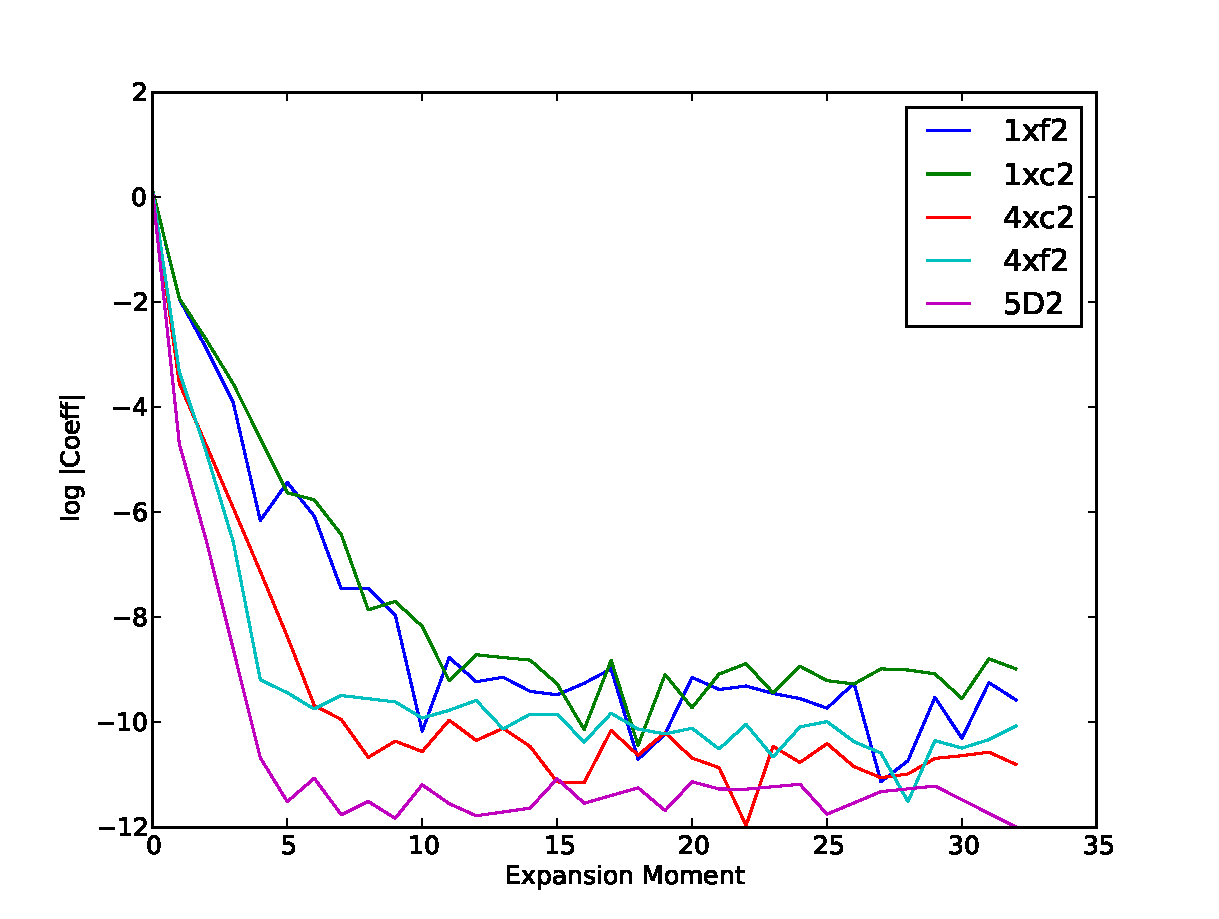
\includegraphics[width=0.7\textwidth]{../graphics/coefficient_decay2}
   \caption{2G2D: Coarse Mesh Coefficient Decay}
   \label{fig:2g2d5v fine cof}
\end{figure}
\begin{table}[H]
\begin{center}
\begin{tabular}{c c c|l l}
type & tol & $\mathcal{P}(\Sigma_{2,c}^1,\Sigma_{2,f}^1,\Sigma_{2,c}^4,\Sigma_{2,f}^4,D^5_2)$ & mean & variance \\ \hline
MC & - & - & 0.999064586714 & 0.0262019588485 \\
SC & 1e-4 & (5, 4, 3, 3, 1) & 1.00191085676 & 0.000202816510815 \\
SC & 1e-5 & (6, 5, 4, 3, 1) & 1.00112487809 & 0.000554497293737\\
SC & 1e-6 & (8, 7, 5, 4, 2) & 1.00018130781 & 0.00245280240592 \\
SC & 1e-8 & (10, 9, 6, 4, 3) & 1.00014901416 & 0.00207327774315
\end{tabular}
\end{center}
\caption{Convergence of Mean, Variance for 2D2G Case, Expansion Tolerances}
\label{tab:informed 5v}
\end{table}
%
%\begin{figure}[h!]
%\centering
%   \includegraphics[width=\textwidth]{../graphics/}
%   \label{}
%   \caption{}
%\end{figure}
%\begin{table}
%\begin{center}
%\begin{tabular}{c c|l l| r}
%type & runs/order & mean & variance & run time (sec) \\ \hline
%MC & 1\times10^6 &  &  & \\
%SC & 2 & & & \\
%SC & 4 & & & \\
%SC & 8 & & & \\
%SC & 16 & & &
%\end{tabular}
%\end{center}
%\caption{}
%\label{}
%\end{table}
%
%\begin{figure}[h!]
%\centering
%   \includegraphics[width=\textwidth]{../graphics/}
%   \label{}
%   \caption{}
%\end{figure}
